\begin{exercise}{Piège de Ioffe--Pritchard}{-1}{Spé}
{}{mines}

\paragraph{Exercice} \textsf{(30 minutes préparation, 25 minutes de passage) \textbf{:}}

On considère les dispositifs suivants qui servent à piéger des atomes :
\begin{center}
    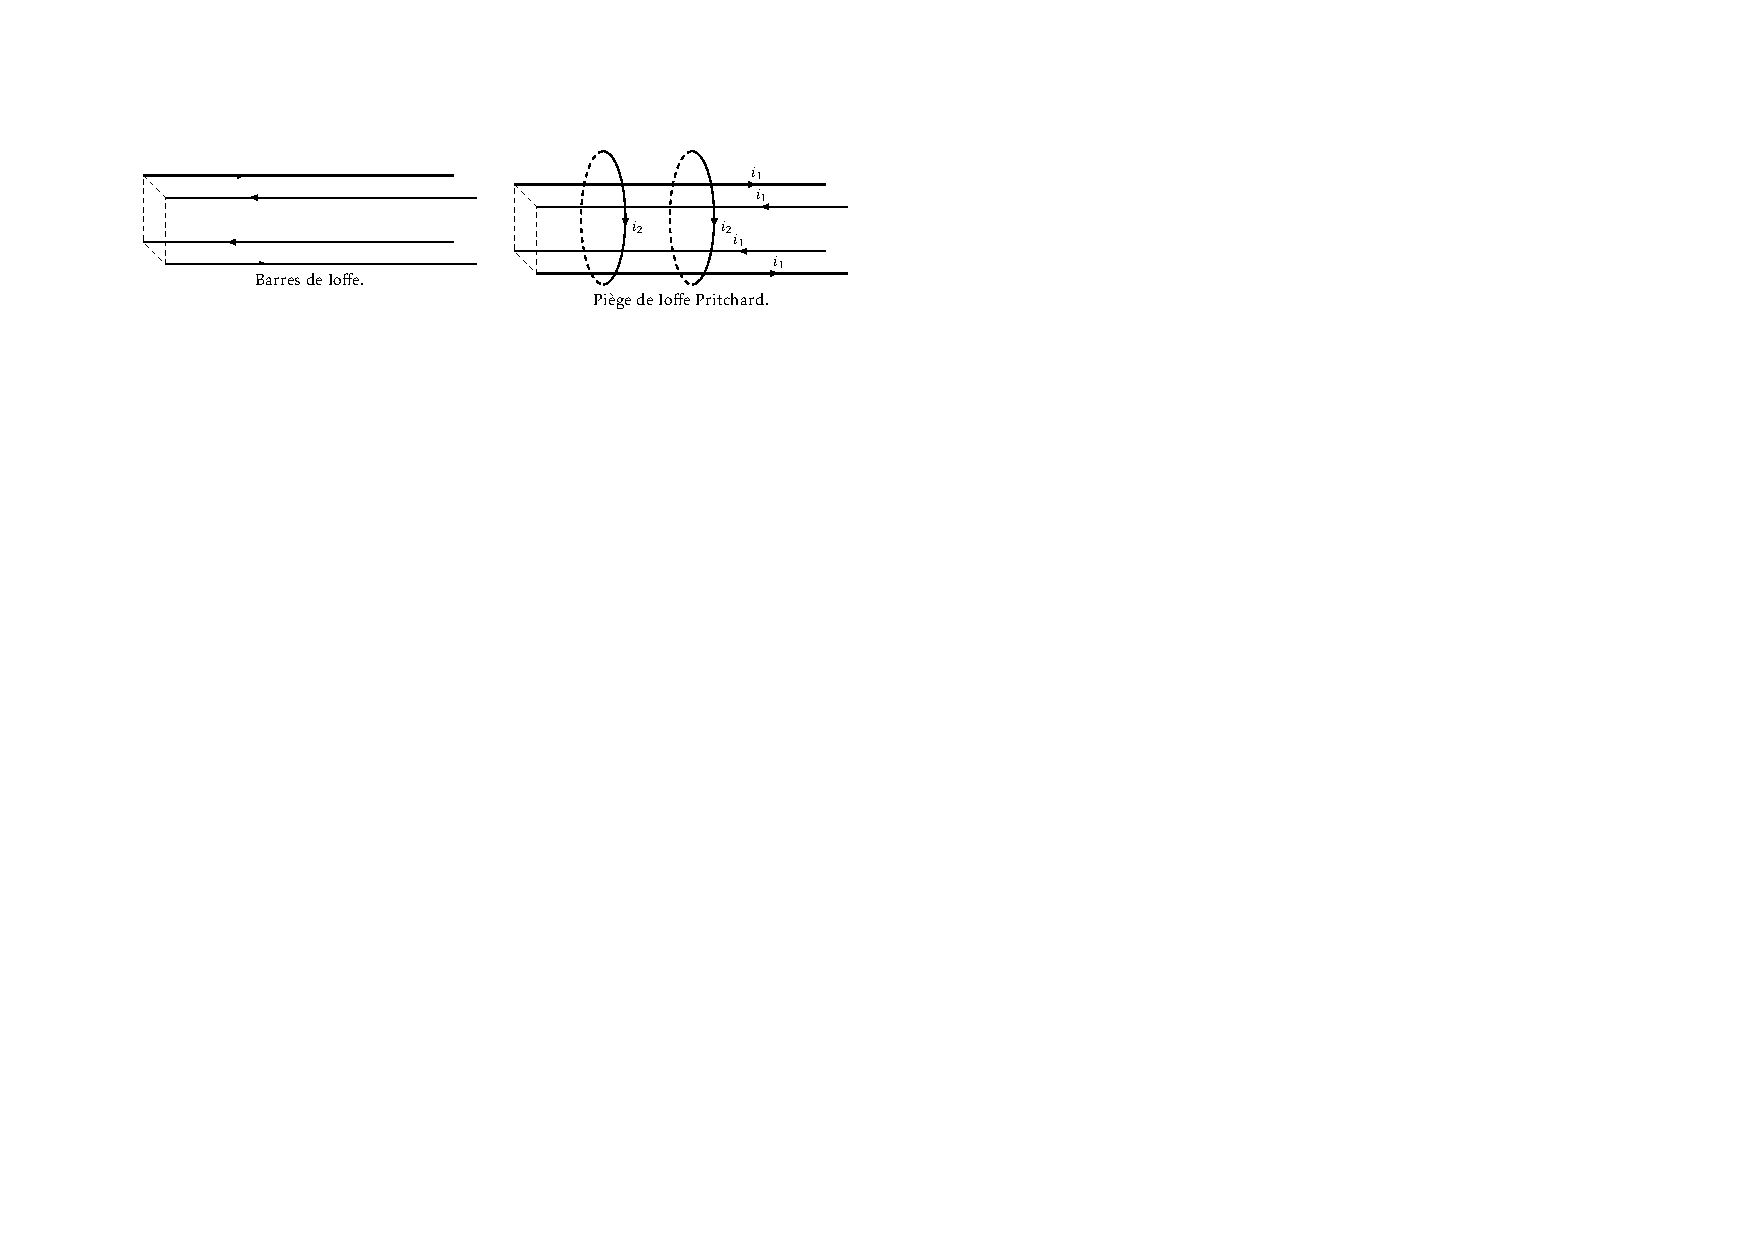
\includegraphics[width=\linewidth]{oraux/mines/Ioffe.pdf}  
\end{center}

\begin{questions}
    \questioncours Redémontrer rapidement l'expression du champ magnétique $b_1$ émis par un fil infini parcouru par un courant $i_1$ le long de l'axe $\ve_z$.
    \question Montrer qu'il peut s'exprimer sous la forme
    $$\vec{b}_1(\vr) = \rot\vec{a}_1 \qqtext{avec} \vec{a}_1(\vr) = a_0\ln (r/r_0)\ve_z,$$
    avec $\vec{a}_1$ un champ qu'on appelle le potentiel vecteur du champ magnétique et $a_0$ une constante dont on donnera l'expression et $r_0$ une constante arbitraire. \vspace{-1em}
    \uplevel{
    \paragraph{Attention :} le potentiel vecteur est une notion hors programme ; il ne sera pas exigé du ou de la candiat$\cdot$e de connaissance à son sujet. On s'en tiendra à la seule définition mathématique $\vB = \rot\vA$.}
    \uplevel{On s'intéresse maintenant au champ magnétique $B_1$ émis par les barres de Ioffe : quatre fils identiques disposés en carré de côté $c$, comme dans la figure ci-dessus. On note $xy$ le plan du carré et $x=0$, $y=0$ le centre du carré. On note $r$ la distance au centre du carré dans le plan $xy$.}
    \question Sans calcul donner l'allure des lignes de champ $B$ dans le plan $xy$. Quelle est la valeur du champ au centre du carré ?
    \question On se place proche de $r=0$ en considérant que $r\ll c$. Calculer le potentiel vecteur du champ magnétique $A_1$ des barres de Ioffe en $\vr$. On prendra la constante $r_0 = c$.
    \question En déduire l'expression pour le champ $B_1$.
    \uplevel{Afin de contraindre également la particule dans la direction des $z$, on ajoute deux spires de rayon $R$ séparées d'une distance $d$ : c'est le piège de Ioffe--Pritchard.}
    \question 
    Le champ magnétique $b_2$ émis par une seule spire de courant $i_2$ si on se place sur son axe de révolution est
    $$b_2(z) = \dfrac{\mu_0 i_2 R^2}{2(R^2+z^2)^{3/2}}.$$
    Au vu de vos connaissances sur les symétries du champs magnétique et sur les dipôles magnétiques, interpréter cette expression.
    \question En supposant que l'on soit proche du milieu des deux spires et sur leur axe de révolution, calculer le champ magnétique $B_2$ émis par les deux spires.
    \question Lorsqu'on somme $B_1$ et $B_2$, quel type de profil de champs magnétique a-t-on ? Interpréter en terme de trajectoire d'une particule chargée proche du centre.
\end{questions}

\paragraph{Données} $\rot$ est l'opérateur rotationnel dont l'expression en coordonnées cylindriques est
$$\rot\vec{a} = \qty(\dfrac{1}{r}\pdv{a_z}{\theta} - \pdv{a_\theta}{z})\ve_r +\qty(\pdv{a_r}{z} - \pdv{a_z}{r})\ve_\theta + \dfrac{1}{r}\qty(\pdv{(ra_\theta)}{r} - \pdv{a_r}{\theta})\ve_z$$

\end{exercise}
